\chapter{Introduction to the problem}
\label{ch:introduction_to_the_problem_mongodb}%
In this part, we implement a bibliographic database through MongoDB, which is a document-oriented database.
In the previous part, using Neo4j, the main focus was on the relationships between nodes, instead, MongoDB's paradigm is different.
It shifts the attention to the document itself, which is the atomic and fundamental element of the database.
In this case, each document represents a single paper and contains all the related information.
All the articles are stored in the same collection called \verb|bibliography|.
A bibliographic database is a use case where the documental approach may be very successful.
The main focus of this kind of database is to store the information regarding every single paper without the need to relate many articles together and without doing very complex queries.


\chapter{Document structure}
\label{ch:document_structure_mongodb}%
Since we are using a documental database, papers are the main entity and, because of this, it is reasonable to store the text and the structure of the articles.
These fields are added to the attributes listed in the previous part regarding graph databases.
In particular, each paper is composed of many sections and each section has a title, several paragraphs, and a certain number of image URLs with associated captions.
Moreover, each section can contain subsections that have the same structure as a section.

In addition, also the email and bio of the authors have been added as well as the publication date of the article.

The following table shows the document's fields associated with their respective MongoDB type and meaning.
\begin{table}[H]
    \centering
    \begin{tabular}{| c | c | c |}
        \hline % \rowcolor{bluepoli!40}
        \textbf{Field name}      & \textbf{Type}   & \textbf{Description} \T\B \\
        \hline \hline
        \_id                     & String          & paper ID\T\B              \\
        title                    & String          & paper title\T\B           \\
        authors                  & Array of Object & list of authors\T\B       \\
        authors.\_id             & String          & author ID\T\B             \\
        authors.name             & String          & author name\T\B           \\
        authors.org              & String          & author affiliation\T\B    \\
        authors.email            & String          & author email\T\B          \\
        authors.bio              & String          & author short bio\T\B      \\
        keywords                 & Array of String & paper keywords\T\B        \\
        fos                      & Array of String & paper fields of study\T\B \\
        publication\_type        & String          & paper type\T\B            \\
        venue                    & String          & publication name\T\B      \\
        volume                   & Int32           & journal volume\T\B        \\
        issue                    & Int32           & journal issue\T\B         \\
        page\_start              & Int32           & start page\T\B            \\
        page\_end                & Int32           & end page\T\B              \\
        date                     & Date            & publication date\T\B      \\
        lang                     & String          & paper language\T\B        \\
        isbn                     & String          & book ISBN\T\B             \\
        issn                     & String          & journal ISSN\T\B          \\
        doi                      & String          & paper DOI\T\B             \\
        publisher                & String          & publisher name\T\B        \\
        location                 & String          & conference location\T\B   \\
        abstract                 & String          & paper abstract\T\B        \\
        url                      & Array of String & paper URLs\T\B            \\
        references               & Array of String & paper references\T\B      \\
        sections                 & Array of Object & paper sections\T\B        \\
        sections.title           & String          & section title\T\B         \\
        sections.paragraphs      & Array of String & section paragraphs\T\B    \\
        sections.subsections     & Array of Object & section subsections\T\B   \\
        sections.figures         & Array of Object & section figures\T\B       \\
        sections.figures.URL     & String          & figure URL\T\B            \\
        sections.figures.caption & String          & figure caption\T\B        \\
        \hline
    \end{tabular}
    \\[8pt]
    \caption{Description of the fields with related type and meaning.}
    \label{tab:document_structure_mongodb}%
\end{table}
Notes:
\begin{itemize}
    \item \verb|publication_type| can only assume ``Journal'', ``Book'' or ``Conference'' as value;
    \item a paper of type ``Journal'' can have the fields \verb|issn|, \verb|volume|, \verb|issue| and \verb|publisher|;
    \item a paper of type ``Book'' can have the fields \verb|isbn| and \verb|publisher|;
    \item a paper of type ``Conference'' can have the field \verb|location|;
    \item \verb|subsections| have the same structure as \verb|sections|, so they could contain multiple \verb|subsections| and so on in a recursively way.
    We decided to consider only one level of subsections, so \verb|subsections| don't have the \verb|subsections| field.
\end{itemize}
The following code snippet shows our document structure represented in JSON format.
\begin{lstlisting}[label={lst:document_structure_mongodb}]
{
    "_id": <String>,
    "title": <String>,
    "authors": [
        {
            "_id": <String>,
            "name": <String>,
            "email": <String>,
            "bio": <String>,
            "org": <String>
        }
    ],
    "abstract": <String>,
    "keywords": [<String>],
    "fos": [<String>],
    "publication_type": <String>,
    "venue": <String>,
    "volume": <Int32>,
    "issue": <Int32>,
    "issn": <String>,
    "publisher": <String>,
    "isbn": <String>,
    "location": <String>,
    "date": <ISODate>,
    "page_start": <Int32>,
    "page_end": <Int32>,
    "lang": <String>,
    "doi": <String>,
    "url": [<String>],
    "references": [<String>],
    "sections": [
        {
            "title": <String>,
            "paragraphs": [<String>],
            "figures": [
                {
                    "URL": <String>,
                    "caption": <String>
                }
            ],
            "subsections": [
                {
                  "title": <String>,
                  "paragraphs": [<String>],
                  "figures": [
                      {
                          "URL": <String>,
                          "caption": <String>
                      }
                  ]
                }
            ]
        }
    ]
}
\end{lstlisting}
Below we provide some examples of the three main paper types that appear in our document with their associated attributes.
The difference in the attributes is minimal and, as mentioned beforehand, it concerns the fields related to the publishing type of the paper.

\paragraph{Model of journal:}
This is the document structure for the papers published in journals.
\begin{figure}[H]
    \begin{center}
        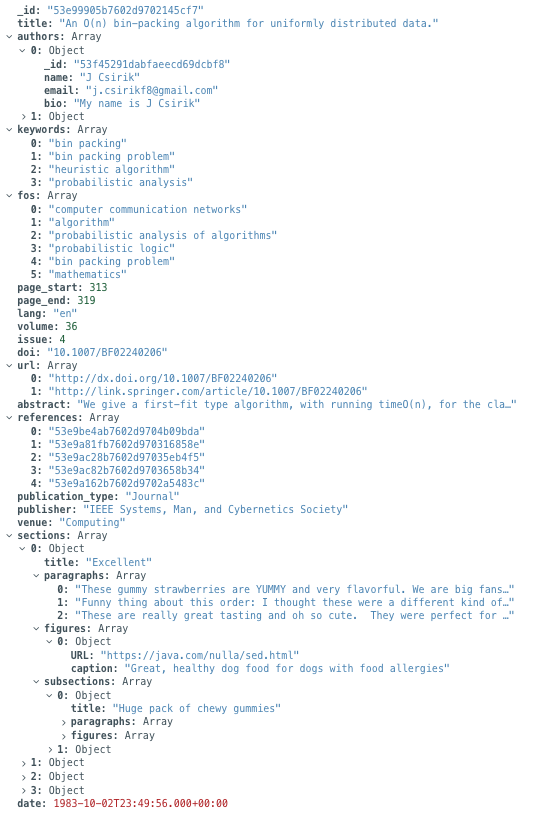
\includegraphics[width=0.9\linewidth]{ImagesMongoDB/journal}
        \label{fig:journal}%
    \end{center}
\end{figure}

\paragraph{Model of book:}
This is the document structure for the papers published in books.
\begin{figure}[H]
    \begin{center}
        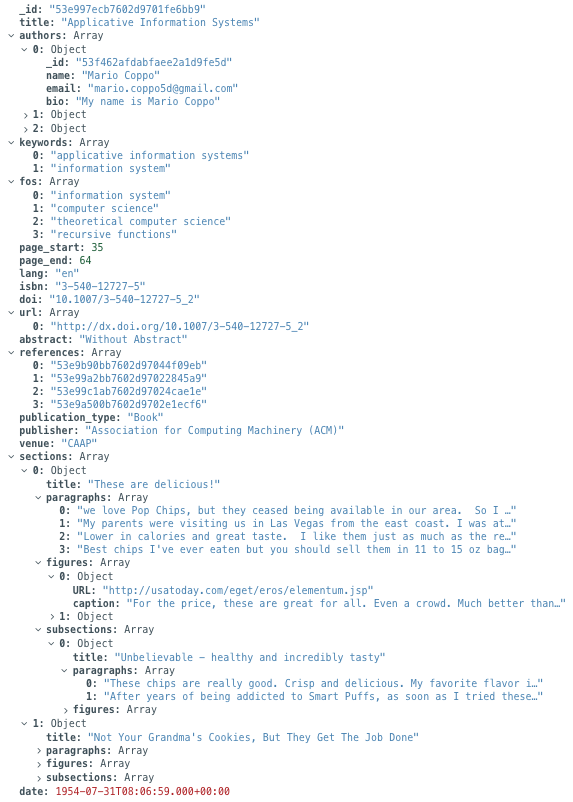
\includegraphics[width=0.9\linewidth]{ImagesMongoDB/book}
        \label{fig:book}%
    \end{center}
\end{figure}

\paragraph{Model of conference:}
This is the document structure for the papers published at conferences.
\begin{figure}[H]
    \begin{center}
        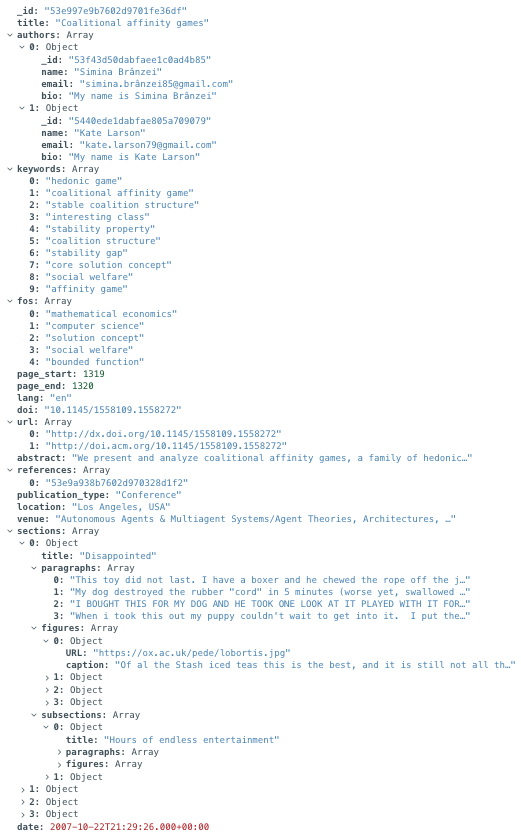
\includegraphics[width=0.9\linewidth]{ImagesMongoDB/conference}
        \label{fig:conference}%
    \end{center}
\end{figure}


\section{Differences concerning the previous models}
\label{sec:differences_concerning_the_previous_models}%
The main advantage of this approach is the fact that it is very easy to get all the relevant data of an article because all the information is stored together and usually allows to avoid performing expensive joins that would be necessary using a relational database.

Furthermore, MongoDB is flexible permitting to have heterogeneous documents, we need to maintain the same skeleton for all documents in the same collection to perform meaningful queries and have a clean database, but also differences between documents are admitted.
As highlighted in the notes above, different types of articles can have different fields and if an article doesn't have certain data is not necessary to store an empty field, simply the attribute is not created.
In addition, this flexibility makes easy the storage of the text structure that could, in principle, have many levels of subsections.

One drawback is the duplication of data, for example, an author may have written more than one paper that is stored in the database, so the author's information is saved multiple times.
This situation could lead to some inconsistency and requires attention when data updates are performed.
But, in the field of bibliography, it is seldom necessary to do updates since all data refer to a specific article and if a paper is modified it is more probable to create a new document with the new version than update the older one.


\chapter{Data upload}
\label{ch:data_upload_mongodb}%


\section{Pre-processing}
\label{sec:pre_processing_mongodb}%
The assignment for this part of the project defined a basic structure of the document with the fields it must have.
Some of the fields defined by this structure were not present in our previous dataset so we had to fix this aspect by doing some pre-processing of the data before working with it.
The starting point has been the dblp dataset, cleaned with python scripts just like in the Neo4j part, but also enriched with new information and new filters on the data.
In particular, the main work revolved around the following fields.

\paragraph{Author email and bio}
Using a Python script, we added the emails of the authors adopting the following format:
\begin{lstlisting}[label={lst:author_email}]
author.name + last-two-digits-of-the-author._id + "@gmail.com"
\end{lstlisting}
Using the same script, we added the bio using the format:
\begin{lstlisting}[label={lst:author_bio}]
"My name is " + author.name + "." + "I'm currently working for " + author.org
\end{lstlisting}
The second sentence, \verb|'"I'm currently working for " + author.org'| is present only if the author has an affiliation.

Then we generated random dates adopting the format \verb|ISODate| of \verb|MongoDB| from \href{https://www.mockaroo.com}{mockaroo.com} and added them to the original dataset with a Python script.

\paragraph{Sections and subsections}
The sections and subsections fields, as mentioned in the assignment instructions were mandatory for the document structure.
However, the documents in our dataset didn't have those fields so we had to manually generate them.
We did so by using a Python script.
More specifically the titles of the sections and subsections and the text for the paragraphs were extracted from the fields \verb|Summary| and \verb|Text| respectively, present in an external dataset named \verb|Reviews.csv|\footnotemark\footnotetext{Amazon Fine Food Reviews, accessed on the 14/11/2022\\
\indent\indent https://www.kaggle.com/datasets/snap/amazon-fine-food-reviews}, which consists of food reviews from Amazon.
The script first generates a set of unique sections with a random number of paragraphs and a random number of subsections, which are themselves sections but without a subsections field (the boundaries of this random number were tuned in the script).
We decided to maintain only a level of subsections to have a more concise document that satisfies the requirements.
Secondly, a (bounded) random number of sections were added to each paper document of the original dataset.

\paragraph{URLs and captions} Images URLs have been generated from \href{https://www.mockaroo.com}{www.mockaroo.com}, while captions are from the \verb|Summary| field of the same dataset \verb|Reviews.csv| used to generate the sections.
We wrote a Python script to add both values to the original dataset.

\paragraph{Venue} The \verb|venue| field was generated from the \verb|venue.raw| given by the initial dataset.
In the version of the \verb|dblp| that we downloaded the venue was a composed field with a lot of information, such as the \verb|raw|, the \verb|name|, the \verb|_id|, and the \verb|type|.
We chose to maintain only the \verb|raw|, which encoded the more interesting data and we assigned it to the field named \verb|venue|.


\section{Upload process}
\label{sec:upload_process_mongodb}%
The upload of the data was quite straightforward since our dataset was already in JSON format.
Since the importing feature of MongoDB was much more efficient than Neo4j we were able to load a much bigger dataset containing 56K documents.

After uploading the data we performed the following filters:
\begin{itemize}
    \item We deleted some fields from all the documents because we were not interested in maintaining all the data, but just the ones that matched more or less the chosen structure for the collection.
    We used the \verb!$unset! command to remove specific fields, such as the \verb|pdf| and the \verb|year|, that was superfluous having the field \verb|date|.
    An example of this procedure is reported in the third command of the following section.
    \item We checked all the fields to remove empty fields, so we cleaned the dataset by removing uninteresting values.
    We executed this cleaning part firstly by checking if the field equals the empty value \verb|""| and then using the \verb|$unset| command on the respective element.
    As before we can see an example of this procedure also in the third command of the following section.
    \item We executed some additional commands to filter the data, from the \verb|FILTERING| option of \verb|MongoDB Compass|, such as the following one:
    \begin{lstlisting}[label={lst:filtering}]
{$and: [
    { title: { $not: { $regex: '^[1-9]' } }},
    { page_start: { $regex: '^[0-9]+$' }},
    { page_end: { $regex: '^[0-9]+$' }},
    { volume : {$not : { $eq : "null"}}},
    { abstract: {$not : {$eq : "null"}}},
]}
    \end{lstlisting}
    Controls similar to the one just reported can be executed at any time, for instance after acquiring some new data from an external source, to have only documents with interesting values.
\end{itemize}


\chapter{Commands and queries}
\label{ch:commands_and_queries_mongodb}%


\section{Commands}
\label{sec:commands_mongodb}%
\begin{enumerate}
    \item \textbf{Inserting a document} \\
    To insert in our database only one document at a time, we use the following function \verb|insertOne()|, which takes in input one document and inserts it in the DB. If the document does not specify an \verb|_id| field, as is our case, then mongod\footnotemark\footnotetext{mongod is the primary daemon process for the MongoDB system} will add the \verb|_id| field and assign a unique \verb|ObjectId()| for the document before inserting it.
    Since when importing this dataset the \verb|_id| were defined as String we decided to explicit the \verb|_id| creation so we can use the \verb|toString()| method to cast it to a String type and be consistent with the data we loaded from the dataset.
    As shown below, for this example we have retrieved a real-world paper and shaped its information to our document structure.
    Firstly, we searched for the author by name and since we didn't find him, we created a new \verb|_id| for him.
    For text formatting reasons in the preview below, we have omitted the values of the \verb|abstract| and \verb|sections| fields.
    The \verb|references| field is an empty array because all the referenced papers by this one are not present in our DB\@.
    \begin{lstlisting}[label={lst:command1mongodb1}]
db.bibliography.insertOne(
{
    _id: ObjectId().toString(),
    title: "Reinforcement Learning for Improving Agent Design",
    authors: [
        {
            _id: ObjectId().toString(),
            name: "David Ha",
            email: "hadavid@google.com",
            bio: "AI resercher at Google Brain, based in Tokyo, Japan",
            org: "Google Brain"
        }
    ],
    abstract: "...",
    keywords: ["computer science", "ai", "reinforcement learning", "cumulative reward", "joint learning"],
    fos: ["computer science", "ai", "reinforcement learning"],
    publication_type: "Journal",
    publisher: "MIT Press Direct",
    venue: "Artificial Life",
    volume: 25,
    issue: 4,
    issn: "352-365",
    date: ISODate('2019-12-02T10:49:36.000'),
    page_start: 23,
    page_end: 46,
    lang: "en",
    doi: "doi.org/10.1162/artl_a_00301",
    url: [
        "https://arxiv.org/abs/1810.03779",
        "https://arxiv.org/abs/1810.03779v3",
        "https://doi.org/10.48550/arXiv.1810.03779"],
    references: [],
    sections: []
})
    \end{lstlisting}
    An easy way to know if the papers referenced by the one we are about to insert are present in the database is to query it using the DOIs of the referenced paper (like is shown in the code snippet below) and then get the \verb|_id| values to be added to the references.
    \begin{lstlisting}[label={lst:command1mongodb2}]
db.bibliography.aggregate([{
    $match: {
        doi: {$in: [
            "10.1109/CMPSAC.2002.1044548",
            "10.1007/s11704-011-0127-6",
            "10.1016/j.datak.2008.09.003"
            ]}}}, {
    $project: {"_id": 1}}
])
    \end{lstlisting}
    Using the database structure presented earlier, we realized that managing the data could not be so straightforward, especially when a new document insertion is required.
    These drawbacks are due to the data sources we had because only a small percentage of the papers had the values for DOI and ORCID but we would have shrunk too much our dataset keeping only those articles.
    In a further improved version, some precautions could be taken to have a more clean and easy-to-use database if the DOI field is known for all documents and the ORCID for all authors.

    With the above assumptions, we could use the DOI for the references because it is a globally unique and independent identifier usable in any database implementation.
    In this way, it would be easier to insert a new document because the new paper could be added to the collection even if the references are not present in the dataset, and the related papers could be inserted afterward.
    Likewise, using the ORCID as the author identifier would also make it easier to add new documents because the ORCID has the same global uniqueness property.
    It would not be necessary to check if the author is already present in the database to set the same id, risking creating inconsistency, but we could insert it just as it is.

    Despite the further checks required in our implementation, when adding the document, we decided to avoid imposing too many limitations on the structure of the data.
    If the papers have the DOI and the authors have the ORCID is easier to search the collection, but we cannot guarantee the presence of these fields, so to have a more flexible database, we accept papers without DOI and ORCID. A less bounded dataset leads to the necessity of adding some checks to maintain data consistency and requires being more careful when inserting data to avoid duplication.
    \item \textbf{Update a single document} \\
    The command \verb|updateOne| allows one to search for a document that matches a specific filter and modifies it accordingly to the update rules expressed inside the query.
    In general, the command modifies only the first found document, but if no document matches the search, then no changes are applied to the database.

    The \verb|$set| operator sets a new value for the specified attribute or creates it if it does not exist.
    The \verb|$unset| operator deletes a specified document attribute if the document has the field otherwise, nothing changes.
    The following command might be useful when new data regarding papers become available or when some information needs to be updated due to mistakes.
    The command allows to find a document with the field \verb|_id| equal to \verb|"53e997bab7602d9701fa09cb"| and changes its field \verb|publication_type| to \verb|"Conference"| because this is its actual type and also changes its field \verb|publisher| to \verb|"Association of Forensic Document Examiners"| with the command \verb|$set|.
    This operator is also used to create the field \verb|location| to which is assigned the value \verb|"Grenoble, France"|.
    The update part of the query also allows the removal of the fields \verb|page_start| and \verb|page_end| by using the command \verb|$unset|.
    \begin{lstlisting}[label={lst:command2mongodb}]
db.bibliography.updateOne( {
    _id: "53e997bab7602d9701fa09cb" }, [ {
        $set: { publication_type: "Conference" } }, {
        $set: { publisher: "Association of Forensic Document Examiners" } }, {
        $set: { location: "Grenoble, France" } }, {
        $unset: [
            "page_start",
            "page_end" ] } ] )
    \end{lstlisting}
    \begin{figure}[H]
        \begin{center}
            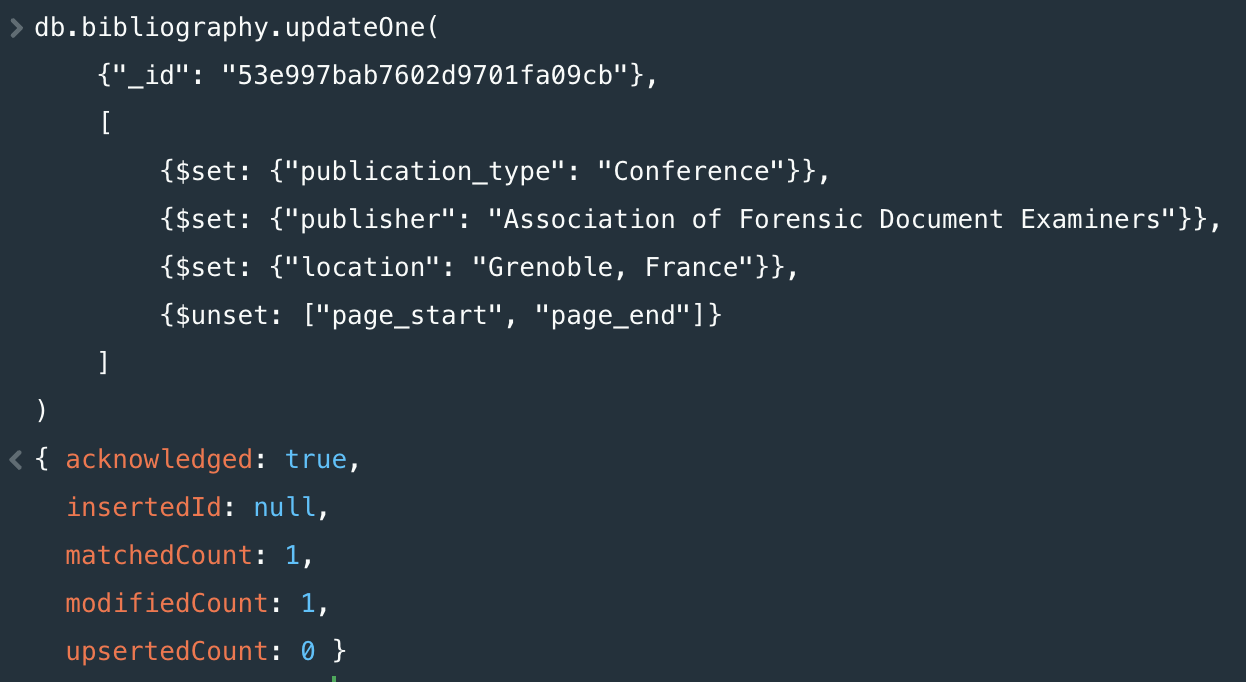
\includegraphics[width=0.9\linewidth]{ImagesMongoDB/command2mongo}
            \label{fig:command2mongodb}%
        \end{center}
    \end{figure}
    In this case, only one document could have been found because the field \verb|_id| is the unique identifier.
    It is necessary to be careful in updating the database in order to avoid updating the wrong documents, deleting fields, and changing important values.

    Another important use case of \verb|updateOne| is associated with the need to replace a document with a different one.
    This exchange can be done using the operator \verb|$replaceWith| and specifying the document to remove and the one that has to be put inside the database instead of it.
    \item \textbf{Remove fields} \\
    Uploading the dataset, as we previously explained in the chapter about the upload process, we ended up with a lot of data, some of which were not of our interest.
    Using the following command we consider all the data entries of the collection \verb|bibliography| and without any filtering, we just remove the \verb|year| field from all the documents.
    We decided to remove this field because we already have the \verb|date| so this is unnecessary.
    \begin{lstlisting}[label={lst:command3mongodb1}]
db.bibliography.updateMany( {
    }, {
    $unset: { year: "" } } )
    \end{lstlisting}
    In order to maintain only interesting values about the papers, we also remove the empty fields.
    It doesn't make sense to keep fields that are equal to an empty value, so, for instance, if \verb|doi| is just an empty string, we delete it from the respective document.
    We keep only useful data that respect the structure of the dataset we want to work with to extract knowledge.
    We executed the following command for all the fields for the sake of having a clear collection.
    \begin{lstlisting}[label={lst:command3mongodb2}]
db.bibliography.updateMany( {
    doi: { $eq: "" } }, {
    $unset: { doi: "" } } )
    \end{lstlisting}
    \item \textbf{Delete a group of documents} \\
    The command \verb|deleteMany()| deletes a group of documents that match the condition given inside the specified filter.
    In this case, the documents that have as date one that occurs before the \verb|1950| are considered obsolete, so we want to delete them.
    For this reason, it's enough to execute a check on the field \verb|date|, that is of date type, so we have to specify the \verb|ISODate| format and delete all the documents previous to \verb|'1950-01-01T00:00:00.000Z'|.
    \begin{lstlisting}[label={lst:command4mongodb}]
db.bibliography.deleteMany( { date: { $lt: ISODate("1950-01-01T00:00:00.000Z") } } )
    \end{lstlisting}
    After executing the command successfully, \verb|MongoDB| acknowledges the write operation and returns the number of documents that were eliminated from the collection.
    \begin{figure}[H]
        \begin{center}
            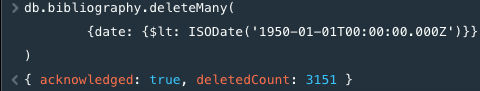
\includegraphics[width=0.6\linewidth]{ImagesMongoDB/delete}
            \label{fig:delete}%
        \end{center}
    \end{figure}
    \item \textbf{Update a group of documents} \\
    The command \verb|updateMany| allows the modification of multiple documents at the same time.
    Since in the database some articles have \verb|"Elsevier"| as \verb|publisher|, and some others have \verb|"Elsevier Ltd."|, and since both values represent the same publisher, we want to merge them.
    With the following command, all documents that have value \verb|"Elsevier Ltd."| in the field \verb|publisher| are retrieved, then the value is changed in \verb|"Elsevier"|.
    \begin{lstlisting}[label={lst:command5mongodb}]
db.bibliography.updateMany( {
    publisher: "Elsevier Ltd." }, {
    $set: { publisher: "Elsevier" } } )
    \end{lstlisting}
    \begin{figure}[H]
        \begin{center}
            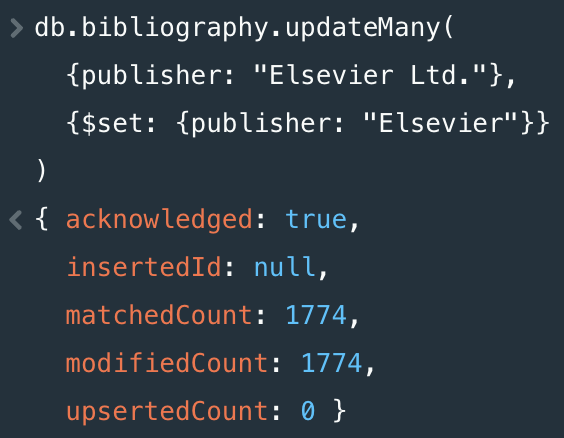
\includegraphics[width=0.45\textwidth]{ImagesMongoDB/command5mongodb}
            \label{fig:command5mongodb}%
        \end{center}
    \end{figure}
\end{enumerate}


\section{Queries}
\label{sec:queries_mongodb}%
\begin{enumerate}
    \item \textbf{Papers published in a certain period on a specific type of publication} \\
    The query's goal is to find all the papers published in a particular time frame delimited by two dates (included) of a type of publication, such as a journal.
    More specifically, the search is conducted on papers published between January 2005 and December 2010 in journals.
    To be compliant with the data type of the \verb|date| field, the date must be specified in a \verb|ISODate| format.
    In the projection, we only show \verb|title| and \verb|venue| of a paper, that is the name of the Journal, and we suppress the field \verb|_id| because not informative.
    \begin{lstlisting}[label={lst:query1mongodb}]
db.bibliography.find( {
    $and: [ {
        date: { $gte: ISODate('2005-01-01T00:00:00.000Z') } }, {
        date: { $lte: ISODate('2010-12-31T00:00:00.000Z') } }, {
        publication_type: "Journal" } ] }, {
    _id: 0,
    title: 1,
    venue: 1 } ).limit(5)
    \end{lstlisting}
    \begin{figure}[H]
        \begin{center}
            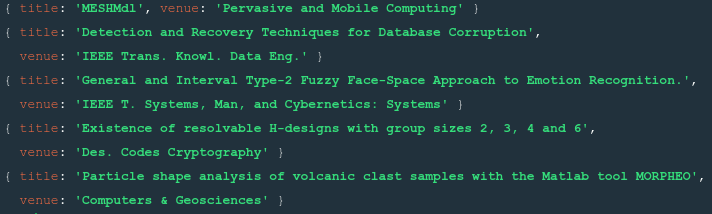
\includegraphics[width=0.9\linewidth]{ImagesMongoDB/query1mongodb}
            \label{fig:query1mongodb}%
        \end{center}
    \end{figure}

    \paragraph{Performance:}
    It's obvious to see that this query iterates through the values of a field to filter some documents.
    If the time range inserted to do the query is small, we can say that the query is highly selective, that is, a query that returns only a few documents from the whole set of scanned documents.
    Selective queries are the ones that make the best usage of indexes, so we thought to do a comparison test of the performance of the query with and without an index on the date.\\
    To have a more meaningful result for the test we removed the \verb|db.collection.limit()| function, otherwise, the automatic rearrangement of the queries would limit the query to stop as soon as it matches 5 correct instances.
    With this limit on the query, the load on the system would be so light that we would see a negligible difference between the query run with and without the indexes.\\
    To get information about the query performance we use \verb|db.collection.explain()|, which returns information about the query plan.
    Passing the \verb|executionStats| argument to this method makes it return an additional section where a set of useful performance markers are shown.

    \paragraph{Results}
    We first try running the query without an index on the field \verb|date|.
    Using the method \verb|explain| with the argument \verb|executionStats| we get the following result (we show only a selection of the markers present in the \verb|executionStats| section, the ones meant for this discussion):
    \begin{figure}[H]
        \begin{center}
            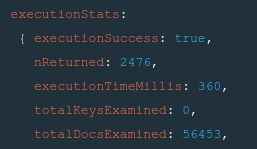
\includegraphics[width=0.45\linewidth]{ImagesMongoDB/result_query1mongodb1}
            \label{fig:result_query1mongodb1}%
        \end{center}
    \end{figure}
    MongoDB runs the query optimizer to choose the winning plan, executes the winning plan to completion, and returns statistics describing the execution of the winning plan.
    In the reported results we can see different parameters that explain the query, and among these, we focus our comparison, especially on the following:
    \begin{itemize}
        \item \verb|nReturned|: number of documents that match the query condition
        \item \verb|executionTimeMillis|: total time in milliseconds required for query plan selection and query execution
        \item \verb|totalKeysExamined|: number of index entries scanned
        \item \verb|totalDocsExamined|: number of documents examined during query execution
    \end{itemize}
    We can clearly see that the documents passing the filter are about 4\% of the total, so we can say that this query is selective enough and can proceed to test it with the addition of an index.
    We'd like also to point out that the \verb|totalKeysExamined| parameter has a value of 0, meaning that this query has not performed a search on indexes.
    Meanwhile, the \verb|totalDocsExamined| shows that all the documents in the DB were examined.
    We proceed to create an index on the field \verb|date| and we run the query again.
    This time the execution plan and stats return different values:
    \begin{figure}[H]
        \begin{center}
            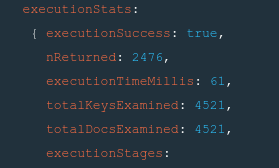
\includegraphics[width=0.45\linewidth]{ImagesMongoDB/result_query1mongodb2}
            \label{fig:result_query1mongodb2}%
        \end{center}
    \end{figure}
    We can immediately notice that the execution time has gone down to 61ms from the 360ms of before, a performance gain of more than 5x.
    Since the indexes are stored in an ordered way the query executioner can iterate through the dates with a much faster binary search algorithm.
    This means we have to do a much smaller number of accesses to the keys of the database, as shown by the value of \verb|totalKeysExamined| parameter in the figure.
    In this particular case, we also have to access the DB (as shown by the \verb|totalDcosExamined| parameter) because the \verb|publication_type| field is not stored in an index, so we have to retrieve the value of this field from the document itself to complete the filtering condition\footnotemark\footnotetext{This type of query, where not all the field needed to compute the query are stored as indexes are called "not covered queries"}.
    Nonetheless, the much lower number of accesses to DB provided by the index on \verb|date| is sufficient to experience a significant gain in performance.
    \item \textbf{Search a given word inside the title of papers written on books and published by a specific publisher} \\
    MongoDB supports query operations that perform a text search, but to enable this functionality is necessary to define a textual index that makes the search possible.

    To achieve more efficient execution of queries, we can define indexes, which are data structures that store useful information to speed up the search.
    When MongoDB executes a query without indexes, it has to evaluate the conditions on all the documents of the considered collection.
    If an index is defined and used, MongoDB can limit the number of analyzed documents and requires less time to compute the results.
    The following command is necessary for creating indexes, and it is essential before executing the following query.
    \begin{lstlisting}[label={lst:query2mongodb1}]
db.bibliography.createIndex( { title: "text" } )
    \end{lstlisting}
    \begin{figure}[H]
        \begin{center}
            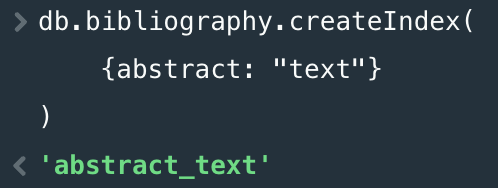
\includegraphics[width=0.45\linewidth]{ImagesMongoDB/query2mongodb1}
            \label{fig:query2mongodb1}%
        \end{center}
    \end{figure}
    Once the index is created, the query can be run.
    It returns the titles of the documents whose title presents the word \verb|"software"| and that were published in a book by the publisher \verb|"Elsevier"|.
    \begin{lstlisting}[label={lst:query2mongodb2}]
db.bibliography.find( {
    $text: { $search: "software" },
    publication_type: "Book",
    publisher: "Elsevier" }, {
    title: 1 } ).limit(5)
    \end{lstlisting}
    \begin{figure}[H]
        \begin{center}
            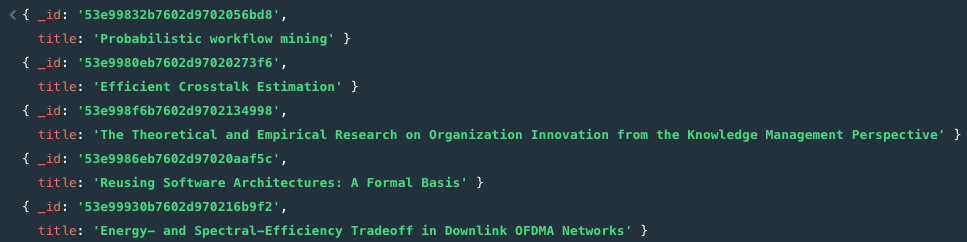
\includegraphics[width=0.9\linewidth]{ImagesMongoDB/query2mongodb2}
            \label{fig:query2mongodb2}%
        \end{center}
    \end{figure}
    \item \textbf{Visualize the common values between the field of study and keywords in each document} \\
    The following query extracts all those documents with at least one keyword as their field of study.

    In particular, we project \verb|title|, \verb|fos|, \verb|keywords|, and their sizes, and then we find all those documents that contain more than thirty keywords, and more than fifteen fields of study.
    We select such a huge number of fields of study and keywords because we are interested in papers that are involved in research that can be important in many areas.

    Finally, we project again \verb|title| and the intersection set between keywords and fields of study to extract and show the ones that match.
    \begin{lstlisting}[label={lst:query3mongodb}]
db.bibliography.aggregate( [ {
    $project: {
        title: "$title",
        fos: "$fos",
        keywords:"$keywords",
        fosSize: { $size: "$fos" },
        keywordsSize: { $size: "$keywords" } } }, {
    $match: { $and: [ {
        keywordsSize: { $gt: 30 },
        fosSize: { $gt: 15 } } ] } }, {
    $project: {
        title: "$title",
        intersection: { $setIntersection: [
            "$fos",
            "$keywords" ] } } } ] )
    \end{lstlisting}
    \begin{figure}[H]
        \begin{center}
            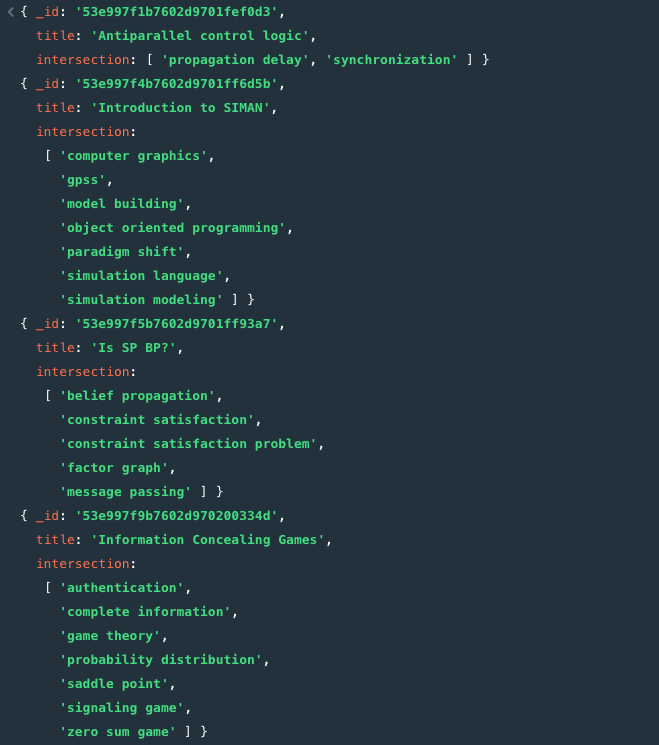
\includegraphics[width=0.9\linewidth]{ImagesMongoDB/query3mongodb}
            \label{fig:query3mongodb}%
        \end{center}
    \end{figure}

    \paragraph{Performance:}
    Let's first consider the query just explained with the relative outcome of the execution, using \verb|explain("executionStats")| in order to analyze its performance:
    \begin{lstlisting}[label={lst:performance_query3mongodb}]
db.bibliography.aggregate( [ {
    $project: {
        title: "$title",
        fos: "$fos",
        keywords:"$keywords",
        fosSize: { $size: "$fos" },
        keywordsSize: { $size: "$keywords" } } }, {
    $match: { $and: [ {
        keywordsSize: { $gt: 30 },
        fosSize: { $gt: 15 } } ] } }, {
    $project: {
        title: "$title",
        intersection: { $setIntersection: [
            "$fos",
            "$keywords" ] } } } ] ).explain("executionStats")
    \end{lstlisting}
    The query firstly scrolls through all the documents, just selecting some fields that we want to project and calculating the size of the \verb|fos| and of the \verb|keywords|.
    In the execution, this is shown by the fact that all the documents that are examined at this first step are also returned.
    This procedure has as \verb|explain.executionStats.| \verb|executionTimeMillis| a value of \verb|633 ms| and doesn't reduce the papers to work on.
    We can also see from the \verb|explain.executionStats.| \verb|totalKeysExamined| that the number of index entries is zero because we don't use any indexing on the fields involved.
    \begin{figure}[H]
        \begin{center}
            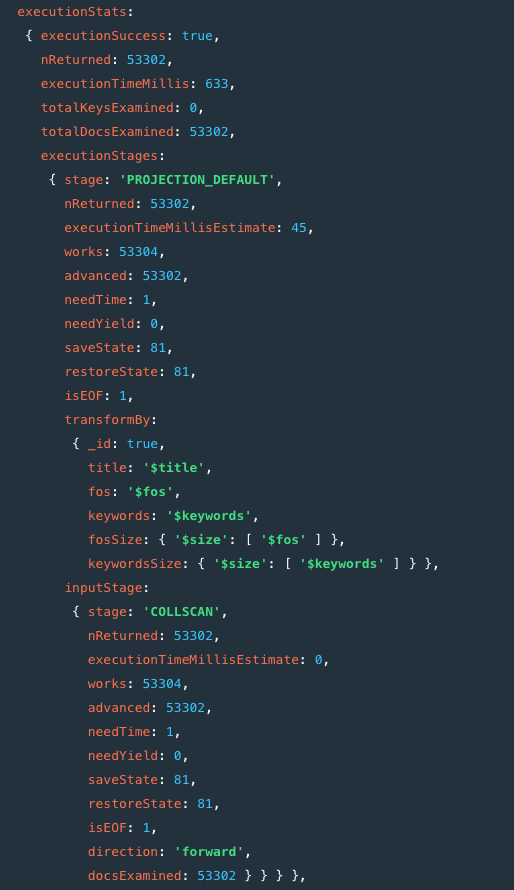
\includegraphics[width=0.6\linewidth]{ImagesMongoDB/performance_query3mongodb1}
            \label{fig:performance_query3mongodb1}%
        \end{center}
    \end{figure}
    After the scrolling, we execute a \verb|match| that narrows down the papers and reduces the computation.
    As follows, we can see that this part of the query requires also \verb|610 ms|, given the fact that has to analyze again all the documents, but after the execution, only \verb|9| matching papers are returned, and shown with the projection.
    \begin{figure}[H]
        \begin{center}
            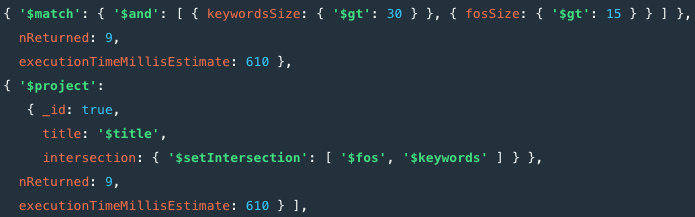
\includegraphics[width=0.9\linewidth]{ImagesMongoDB/performance_query3mongodb2}
            \label{fig:performance_query3mongodb2}%
        \end{center}
    \end{figure}
    Given the fact that the query examined so far has to scroll over all the documents twice, we thought of the following alternative, that first executes the \verb|match| part and then shows the intersection between the \verb|fos| and the \verb|keywords|, without using two projections.
    \begin{lstlisting}[label={lst:performance_query3mongodb3}]
db.bibliography.aggregate( [
    {$match: {
        $expr: {
            $and: [ {
                $gt: [{$size: "$keywords"}, 30 ] }, {
                $gt: [{$size: "$fos"}, 15]
                } ] } } } , {
    $project: {
        title: "$title",
        intersection: { $setIntersection: [
            "$fos",
            "$keywords" ] } } } ] ).explain("executionStats")
    \end{lstlisting}
    As before the query starts examining all the documents of the collection and we have no index entries, not having any index on the involved fields.
    We can see some important differences from the previous procedure looking at mainly two fields of the \verb|explain.executionStats| reported below.
    We can understand from the \verb|explain.executionStats.executionTimeMillis| that the execution time is lower, requiring only \verb|246 ms|, doing the filtering of the papers as the first action of the query.
    Afterward, the projection of the result required only \verb|24 ms|, because the documents were already narrowed down.
    In fact, we can notice that the \verb|match| examined all the collections, but returned only \verb|9| matches, exactly like before, only now this operation was done before any other, so it improved the overall execution.
    \begin{figure}[H]
        \begin{center}
            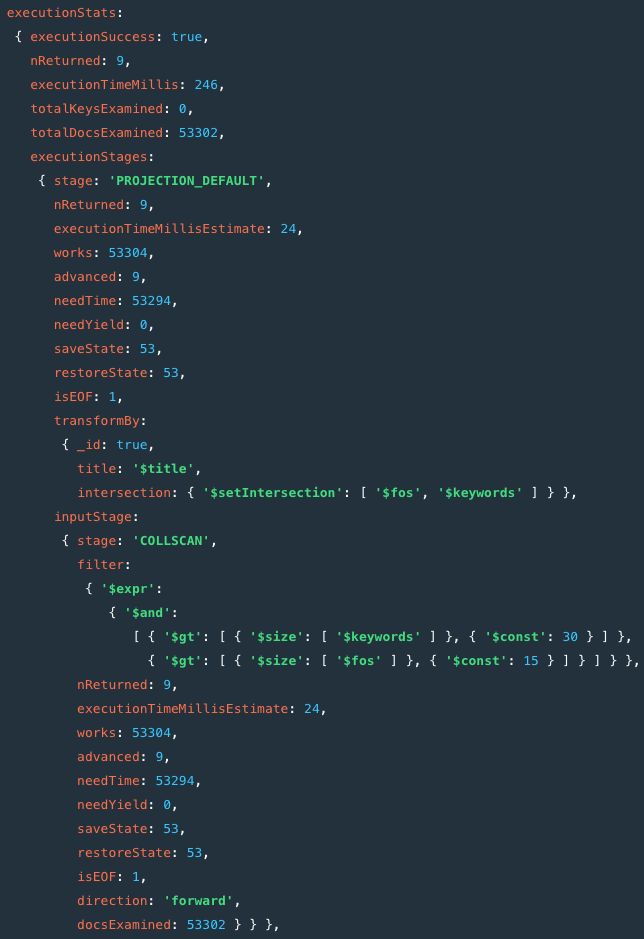
\includegraphics[width=0.6\linewidth]{ImagesMongoDB/performance_query3mongodb3}
            \label{fig:performance_query3mongodb3}%
        \end{center}
    \end{figure}
    In conclusion, this alternative query is more efficient than the previous one, requiring less time to compute.
    From this analysis we noticed that is better to execute the filtering part, the \verb|match|, as soon as possible in the query, in order to reduce the number of documents we have to work on, speeding up the process since the operations are executed like a pipeline.
    \item \textbf{Organizations that held more conferences in the same location} \\
    The following query matches all the papers that are of type \verb|Conference|.
    We select only the events held by the \verb|"IEEE Global Telecommunications Conference| \verb|(Globecom)"| then for each author involved in the conference, we check the affiliation.
    After every step of the query, we obtain a new temporary collection of documents.
    For instance, with the \verb|unwind| command, we deconstruct the array of \verb|authors| from the input papers to output a new document for each element and, in this way, we create a much bigger dataset.

    With this query, we are interested in knowing how many times an organization held a conference in a specific location through one of its members.
    Regrouping the data by conference location and affiliation of the author involved, we can count the number of times the organization took part in an event held there.
    Finally, the result is sorted by the number of engagements and limited only to the first more active organizations.
    \begin{lstlisting}[label={lst:query4mongodb}]
db.bibliography.aggregate( [ {
    $match: { $and: [ {
        publication_type: { $eq: "Conference" } }, {
        venue: { $eq: "IEEE Global Telecommunications Conference (Globecom)" } } ] } }, {
    $unwind: "$authors" }, {
    $group: {
        _id : {
            location: "$location",
            organization: "$authors.org" },
        locationPerOrganization: { $sum: 1 } } }, {
    $project: {
        location: "$location",
        author: "$organization",
        locPerOrgConference: "$locationPerOrganization" } }, {
    $sort: { locPerOrgConference : -1 } }, {
    $limit: 5 } ] )
    \end{lstlisting}
    \begin{figure}[H]
        \begin{center}
            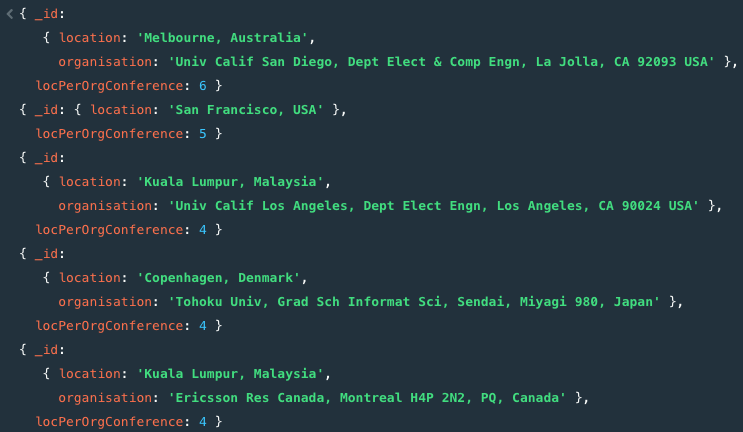
\includegraphics[width=0.9\linewidth]{ImagesMongoDB/query4mongodb}
            \label{fig:query4mongodb}%
        \end{center}
    \end{figure}
    \item \textbf{Papers with a pattern structure} \\
    With this query, we count the number of documents that satisfy a given pattern specified in the \verb|$match| part of the query.
    In this example, we are searching for papers with four sections, and at least one must have four paragraphs, four figures, and one subsection with just one paragraph.
    Using \verb|$size|, it's possible to check the dimension of an array, while using \verb|$elemMatch| is possible to define the criteria that at least one document in an array must satisfy.
    Finally, through the dot notation, we can access a field of an embedded document.
    \begin{lstlisting}[label={lst:query5mongodb}]
db.bibliography.aggregate( [ {
    $match: { $and: [ {
        sections: { $size: 4 } }, {
        sections: { $elemMatch: {
            paragraphs: { $size: 4 },
            figures: { $size:4 },
            subsections: { $size: 1 },
            "subsections.paragraphs": { $size: 1 } } } } ] } }, {
    $group: {
        _id: true,
        count: { $sum: 1 } } } ] )
    \end{lstlisting}
    \begin{figure}[H]
        \begin{center}
            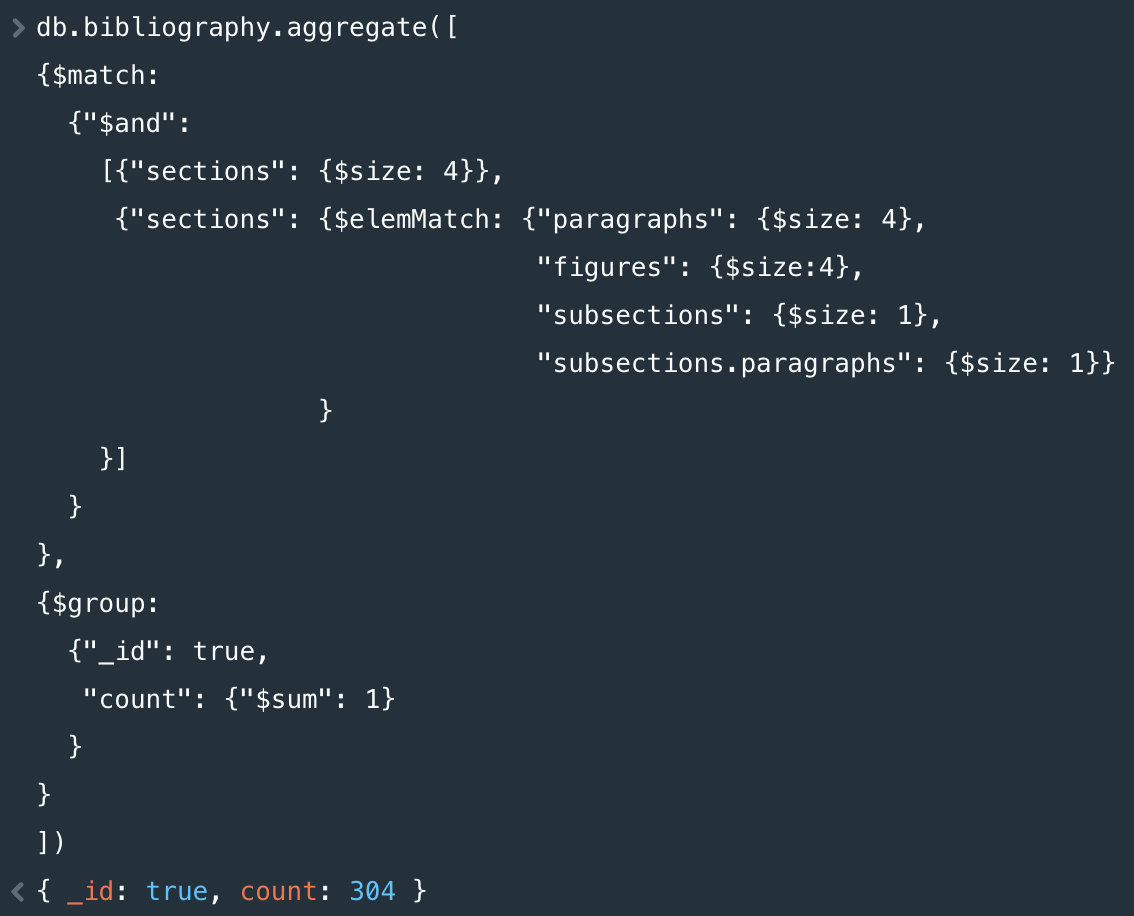
\includegraphics[width=0.6\linewidth]{ImagesMongoDB/query5mongodb1}
            \label{fig:query5mongodb1}%
        \end{center}
    \end{figure}
    \textcolor{red}{The following query is a slight change of the previous one just to retrieve a paper with the wanted structure to show that indeed the query works.}
    \begin{figure}[H]
        \begin{center}
            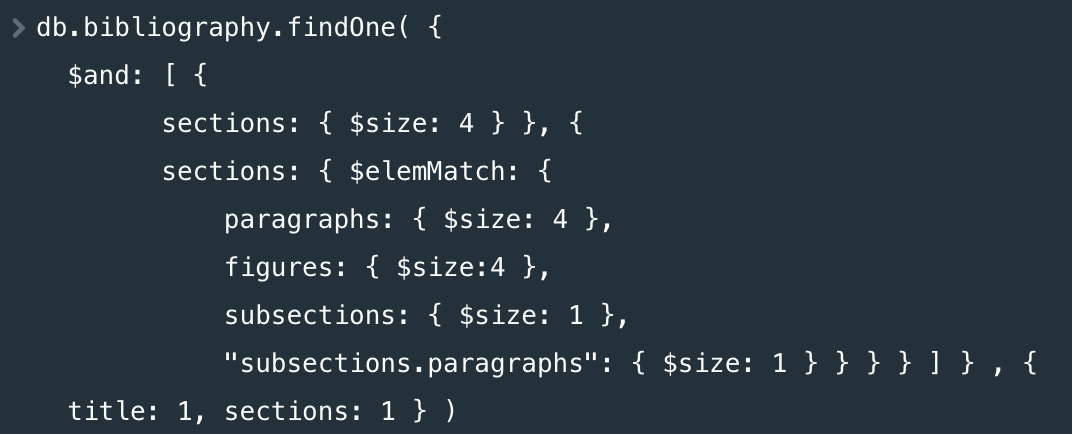
\includegraphics[width=0.6\linewidth]{ImagesMongoDB/query5mongodb2}
            \label{fig:query5mongodb2}%
        \end{center}
    \end{figure}
    \begin{figure}[H]
        \begin{center}
            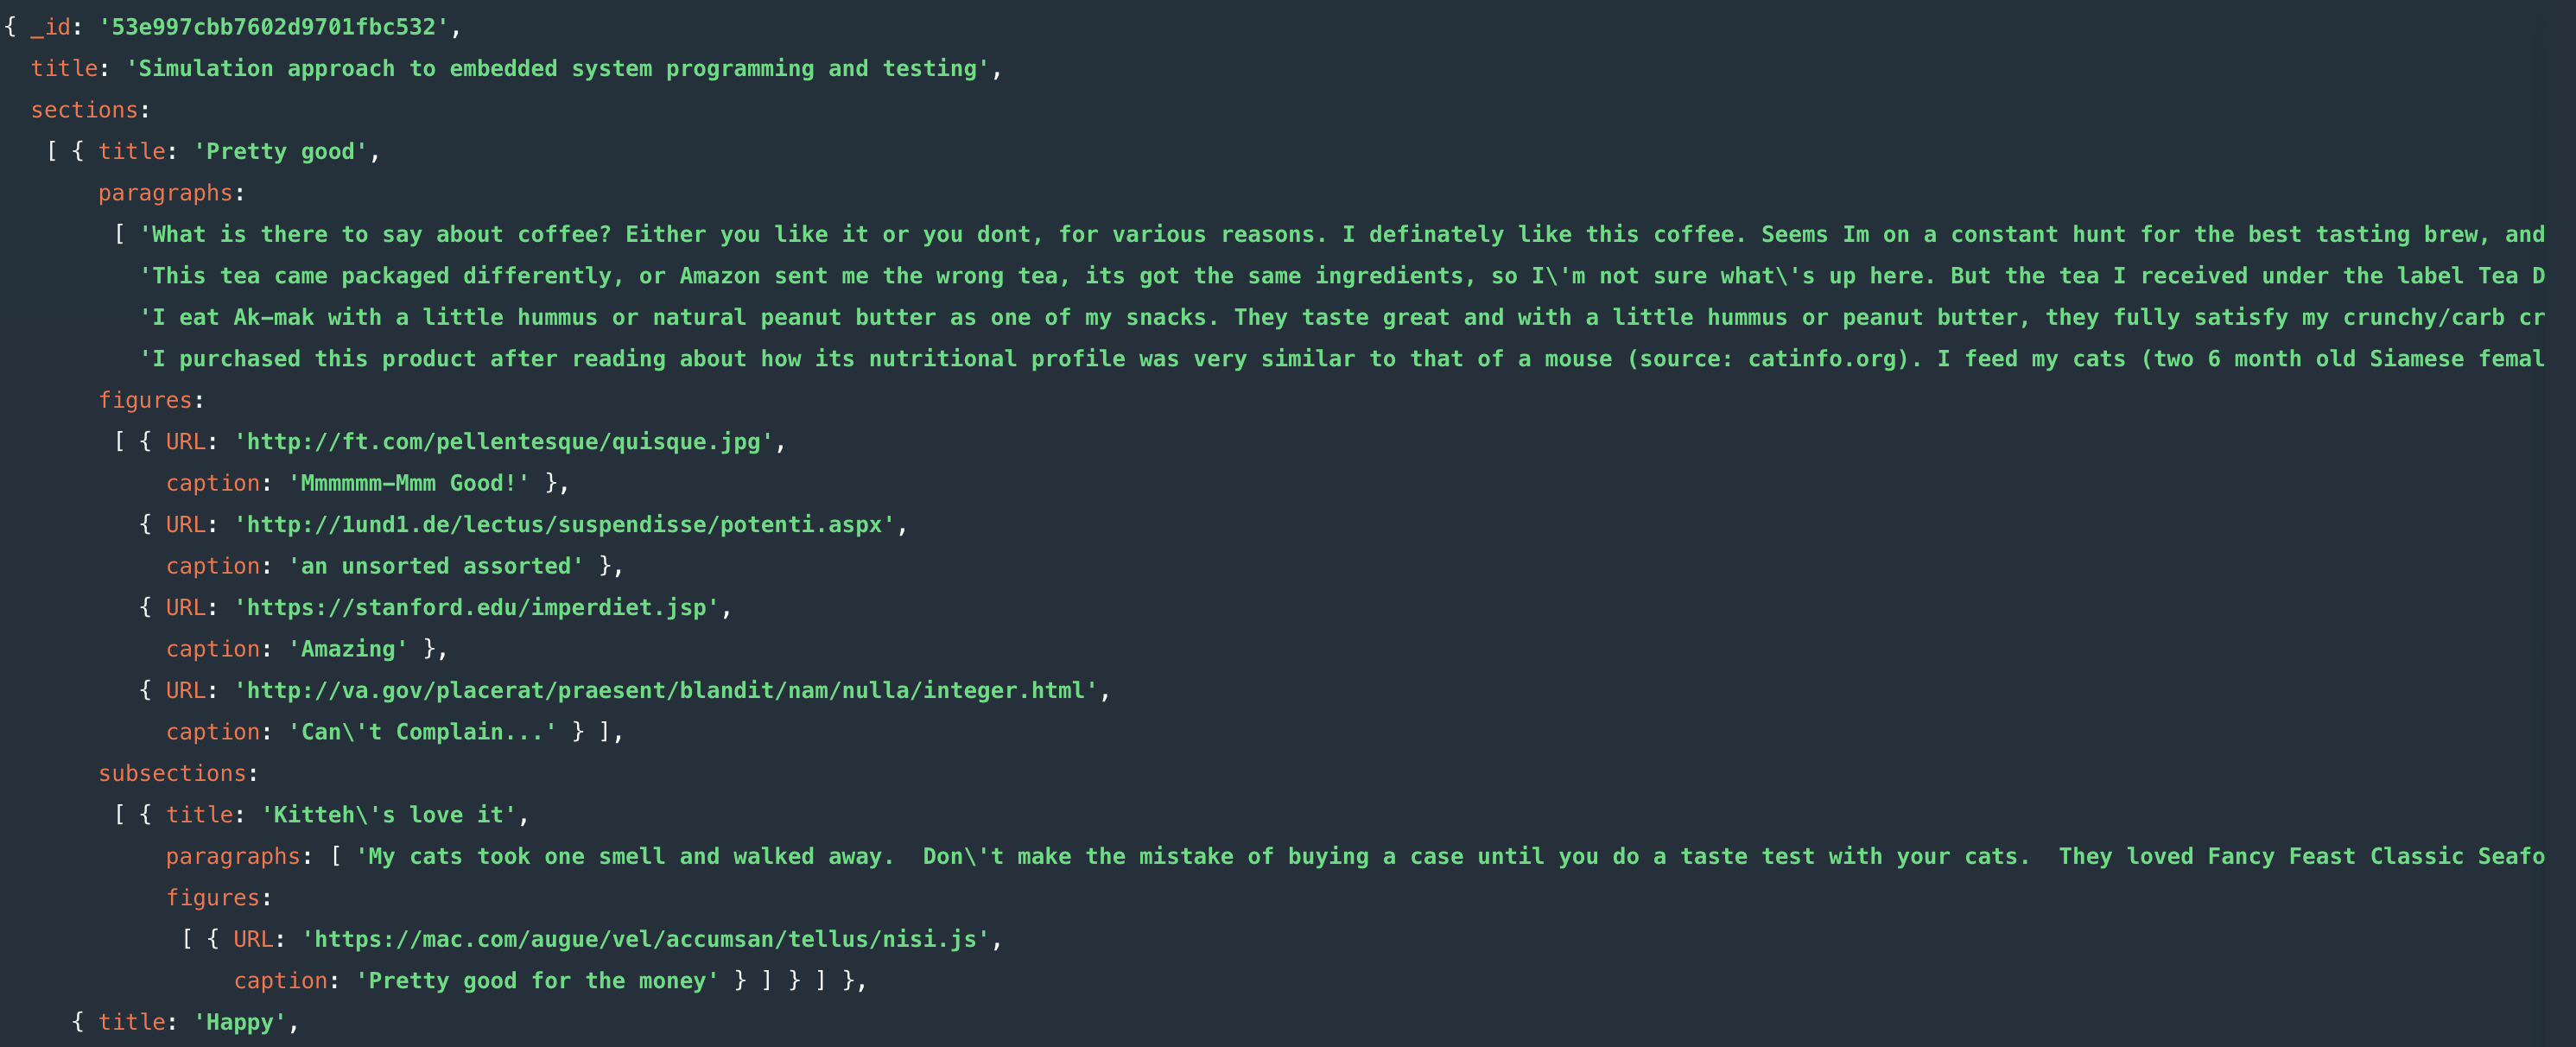
\includegraphics[width=0.9\textwidth]{ImagesMongoDB/result_query5mongodb}
            \label{fig:result_query5mongodb}%
        \end{center}
    \end{figure}
    \item \textbf{Number of papers published by the current staff of an organization} \\
    What we want to achieve with this query is to know how many papers have been published by the researchers working at a certain organization.
    The output list is ordered in descending order, showing the organizations whose researchers have published the most.
    Notice that a paper published by authors from different organizations is counted for all the organizations involved.
    In the first part of the query, we unwind the documents by \verb|authors| and do a filtering of inconsistent data, since the focus of this query is to know which organizations have published the most.
    Secondly, we proceed by grouping documents by the author affiliation (\verb|authors.org|) and the paper itself.
    This operation is needed to filter out the documents referring to the same paper and written by authors that are affiliated with the same organization.
    If we hadn't done this, the same paper would have been counted multiple times, for all the authors who participated in writing it and that are part of the same organization, inflating that organization's contribution.
    Notice that in the result an organization with name \verb|"Corresponding author."| appears, probably this value has been used by the maintainer of the DB to denote independent authors or authors for whom the affiliated organization was not known.
    \begin{lstlisting}[label={lst:query6mongodb}]
db.bibliography.aggregate( [ {
    $unwind: "$authors" }, {
    $match: { $and: [ {
        "authors.org": { $ne: null } }, {
        "authors.org": { $ne: '' } } ] } }, {
    $group: {
        _id: {
            org: "$authors.org",
            p_id: "$_id"} } }, {
    $group: {
        _id: "$_id.org",
        papers: {$sum: 1} } }, {
    $sort: { papers: -1 } }, {
    $limit: 5 } ] )
    \end{lstlisting}
    \begin{figure}[H]
        \begin{center}
            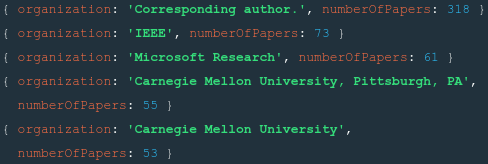
\includegraphics[width=0.9\linewidth]{ImagesMongoDB/query6mongodb}
            \label{fig:query6mongodb}%
        \end{center}
    \end{figure}
    \item \textbf{Number of pages published in Journals by authors affiliated with a certain organization } \\
    This query is similar to the one above, but here we want to retrieve which organizations have contributed the most in writing papers published in journals.
    More specifically, we sum the number of pages written in a specific journal by authors who are currently affiliated with that specific organization.
    This objective is obtained by first unwinding the authors and filtering them to remove some inconsistent data.
    Secondly, we proceed by grouping documents by the author affiliation (\verb|authors.org|) and the paper itself (the other fields of \verb|venue| and \verb|pages| do not contribute to the grouping because they are a single field of the paper document).
    This operation achieves the same goal as the one described in the query before.
    In the second \verb|$group| stage, we group the documents by organization and journal, and we have an accumulator to sum all the pages written by the staff of that organization in that particular journal.
    Finally, the last stages are only for the projection and pretty printing of the output.
    \begin{lstlisting}[label={lst:query7mongodb}]
db.bibliography.aggregate( [ {
    $unwind: "$authors" }, {
    $match: { $and: [ {
        "authors.org": { $ne: null } }, {
        "authors.org": { $ne: '' } }, {
        publication_type: { $eq: "Journal" } }, {
        $expr: { $lte: [
            "$page_start",
            "$page_end" ] } } ] } }, {
        $addFields: { pages: { $subtract: [
            "$page_end",
            "$page_start" ] } } }, {
        $group: { _id: {
            org: "$authors.org",
            paperId: "$_id",
            journal: "$venue",
            pages: "$pages" }, } }, {
        $group: {
        _id: {
            org: "$_id.org",
            journal: "$_id.journal" },
        pages: { $sum: "$_id.pages" } } }, {
    $sort: { pages: -1 } }, {
    $project: {
        organization: "$_id.org",
        journal: "$_id.journal",
        numberOfPages: "$pages" } }, {
    $project: { _id: 0 } }, {
    $limit: 5 } ] )
    \end{lstlisting}
    \begin{figure}[H]
        \begin{center}
            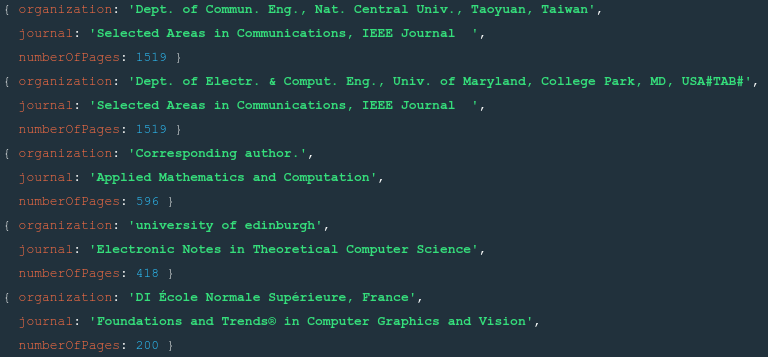
\includegraphics[width=0.9\linewidth]{ImagesMongoDB/query7mongodb}
            \label{fig:query7mongodb}%
        \end{center}
    \end{figure}
    \item \textbf{Couples of the field of study and keyword which appear more frequently within the papers} \\
    The query returns the association between fields of study and keywords which are more present within the database and how many times they appear together.
    Initial filtering is done in order to eliminate the papers which don't contain any keywords or any field of study.
    The two clauses for doing the filtering can be modified by increasing the required number of keywords or the required number of fields of study.
    This kind of change can be interesting in order to understand which fields of study and keywords become more relevant when the subset of the considered paper is different.
    The results are ordered by the number of occurrences of the couples \verb|field of study| - \verb|keyword| by decreasing order.
    This can be done by the operator \verb|"$sort"|.
    We filter out the couples of fields of study and keywords with less than 100 in order to get rid of some misleading information due to not coupled elements.
    The threshold can be adjusted.
    \begin{lstlisting}[label={lst:query8mongodb}]
db.bibliography.aggregate( [ {
    $match: {
        $expr: { $gte: [ { $size: "$fos" }, 0 ] } } }, {
    $match: {
        $expr: { $gte: [ { $size: "$keywords" }, 0 ] } } }, {
    $unwind: { path: "$fos" } }, {
    $unwind: { path: "$keywords" } }, {
    $group: {
        _id: {
            fieldOfStudy: "$fos",
            keyword: "$keywords" },
        keywordsCount: { "$sum": 1 } } }, {
    $match: { "keywordsCount": { $gte: 100 } } }, {
    $sort: { keywordsCount: -1 } }, {
    $limit: 5 }, {
    $project: {
        fieldOfStudy: "$fos",
        keyword: "$keywords",
        score: "$keywordsCount" } } ] )
    \end{lstlisting}
    \begin{figure}[H]
        \begin{center}
            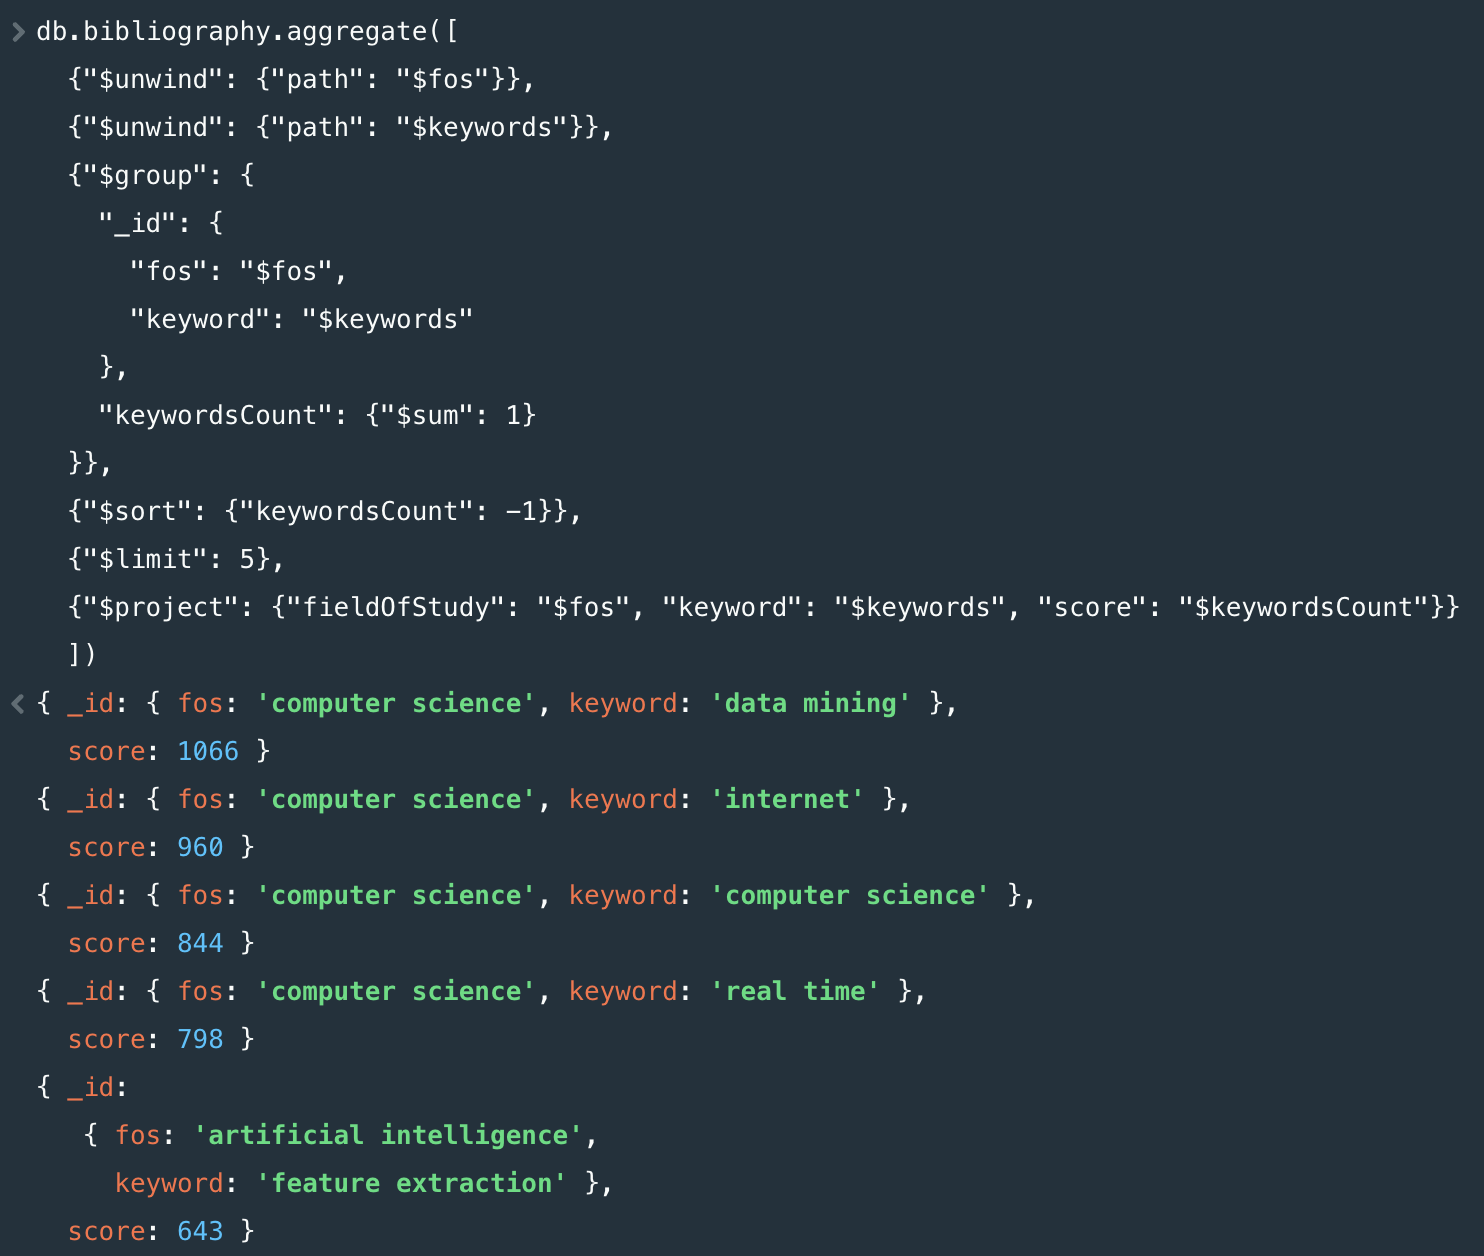
\includegraphics[width=0.9\linewidth]{ImagesMongoDB/query8mongo}
            \label{fig:query8mongodb}%
        \end{center}
    \end{figure}
    \item \textbf{Papers that reference old papers with the same publisher} \\
    In the beginning, we filter the documents retrieving only those that have a \verb|publisher| then, we perform a join between papers and their references using \verb|$lookup| with the condition that the \verb|_id| of the paper must be in the \verb|references| field of the other one.
    In the \verb|$let| command we specify the variables to use in the pipeline that are related to the outer document and that are accessed using \verb|$$|.
    Then we require both papers to have the same publisher and that the referenced article was published at least 10 years before using \verb|$dateDiff|.
    The \verb|_id|, \verb|title|, \verb|publisher|, and \verb|date| of the referenced papers that satisfy these conditions are added to the field called \verb|referencedPapers| in the outer document.
    Lastly, we filter documents keeping only those with at least one joined document, we project only a few fields to make the answer more readable and to check that it is correct, and we limit the number of returned papers.
    \begin{lstlisting}[label={lst:query9mongodb}]
 db.bibliography.aggregate( [ {
    $match: { publisher: { $exists: true } } }, {
    $lookup: {
        from: "bibliography",
        let: {
            pub: "$publisher",
            ref: "$references",
            d: "$date" },
        pipeline: [ {
            $match: { $expr: { $and: [ {
                $in: [
                    "$_id",
                    "$$ref" ] }, {
                $eq: [
                    "$publisher",
                    "$$pub" ] }, {
                $gte: [ {
                    $dateDiff: {
                        startDate: "$date",
                        endDate: "$$d",
                        unit: "year" } },
                    10 ] } ] } } }, {
            $project: {
                _id: 1,
                title: 1,
                publisher: 1,
                date: 1 } } ],
        as: "referencedPapers" } }, {
    $match: { "referencedPapers.0": { $exists: true } } }, {
    $project: {
        _id: 1,
        title: 1,
        publisher: 1,
        date: 1,
        referencedPapers: 1 } }, {
    $limit: 3 } ] )
    \end{lstlisting}
    \begin{figure}[H]
        \begin{center}
            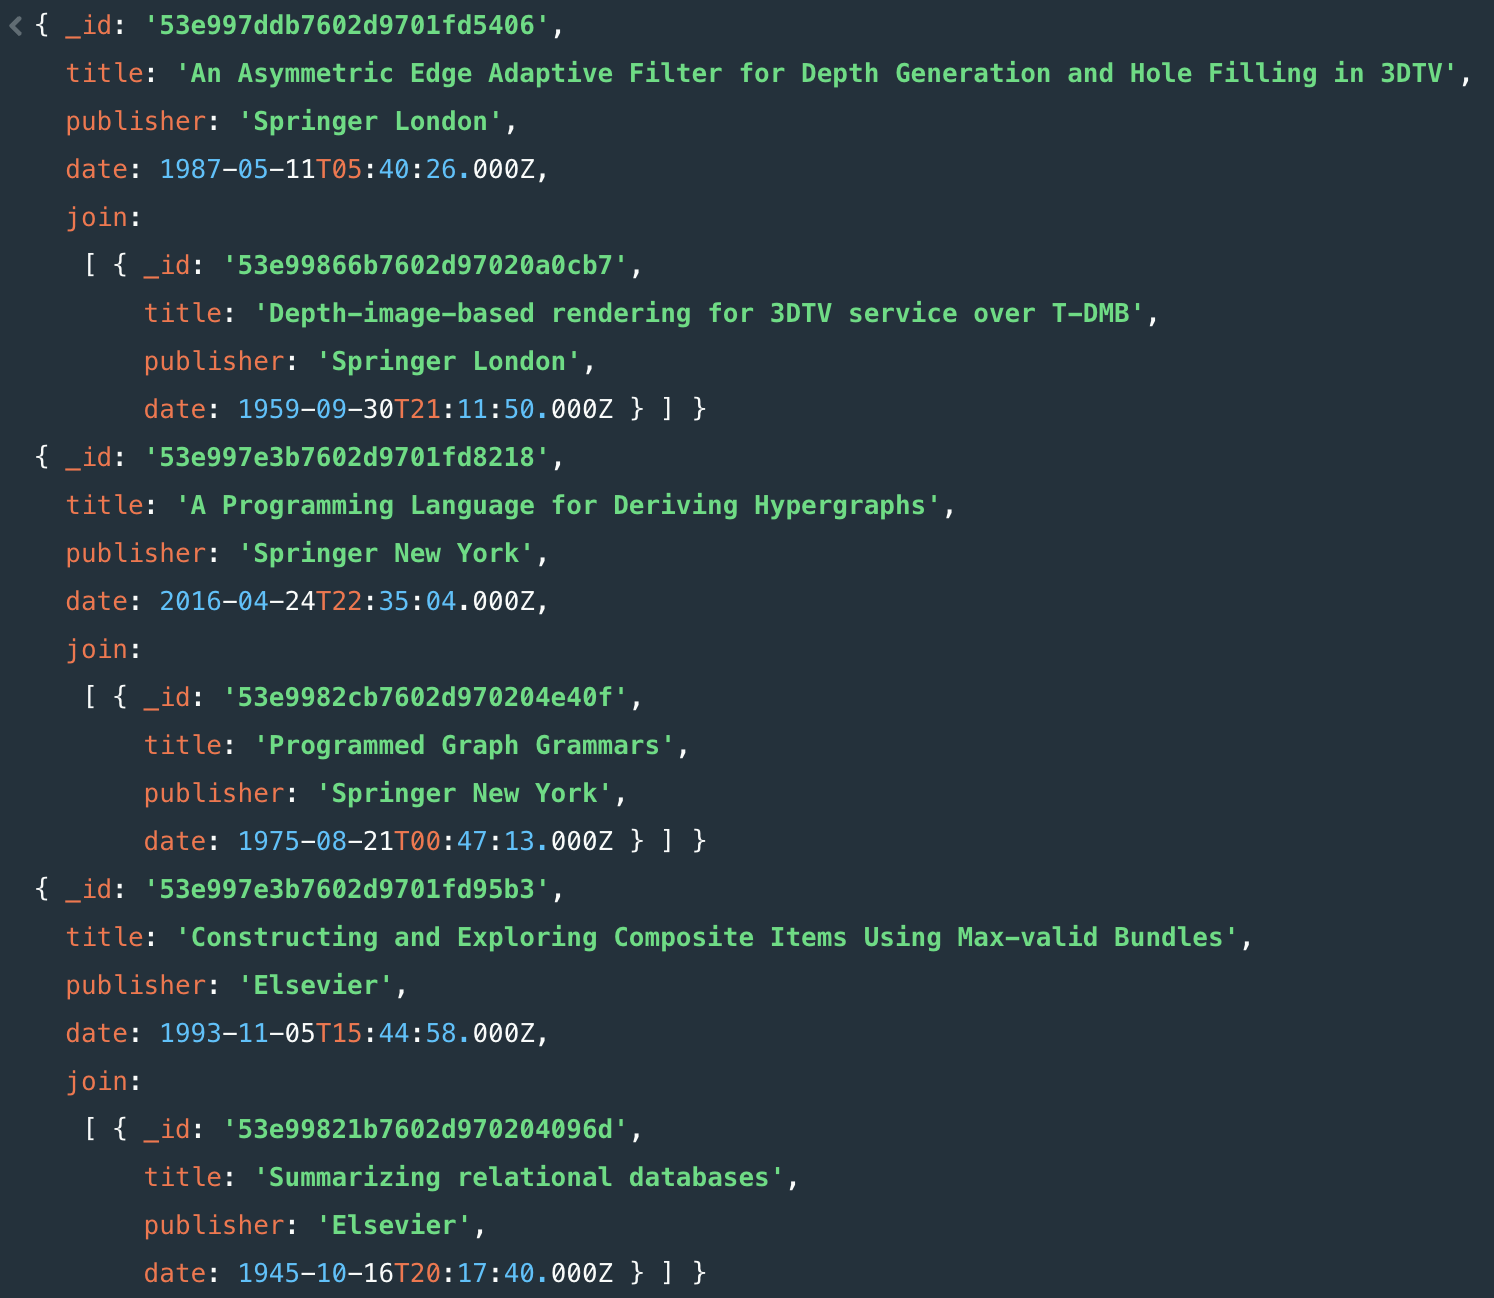
\includegraphics[width=0.9\linewidth]{ImagesMongoDB/query9mongodb}
            \label{fig:query9mongodb}%
        \end{center}
    \end{figure}
    The \verb|$lookup| can be very expensive from a computational point of view and require much time, so to speed the process up it is convenient, when possible, to reduce the input data to the join phase by filtering the documents.
    This can be done by searching for a specific author, title, publisher, or something meaningful in a \verb|$match| condition before the \verb|$lookup|.
    This is possible since all the operations in a query are executed on the database as a pipeline.
    \item \textbf{Recommended books given one book read} \\
    The query returns the book considered the nearest to the given one, in this case, \verb|"Pattern Recognition Letters"|.
    One book is suggested if it has a field of study in common with the book \verb|"Pattern Recognition Letters"|.
    The similarity between books is then evaluated in terms of the number of equal keywords associated with the papers belonging to both considered books.
    \begin{lstlisting}[label={lst:query10mongodb}]
db.bibliography.aggregate( [ {
    $match: { publication_type: "Book" } }, {
    $unwind: { path: "$fos" } }, {
    $unwind: { path: "$keywords" } }, {
    $lookup: {
        from: "bibliography",
        localField: "fos",
        foreignField: "fos",
        as: "otherPaper" } }, {
    $match: { venue: "Pattern Recognition Letters" } }, {
    $unwind: { path: "$otherPaper" } }, {
    $match: { $expr: { $ne: [
        "$_id",
        "$otherPaper._id" ] } } }, {
    $match: { $expr: { $ne: [
        "$venue",
        "$otherPaper.venue" ] } } }, {
    $unwind: { path: "$otherPaper.keywords" } }, {
    $match: { $expr: { $eq: [
        "$keywords",
        "$otherPaper.keywords" ] } } }, {
    $group: {
        _id: { suggestedBook: "$otherPaper.venue" },
        keywordsCount: { $sum: 1 } } }, {
    $sort: { keywordsCount: -1 } }, {
    $limit: 10 }, {
    $project: {
        title: "$suggestedBook",
        similarity: "$keywordsCount" } } ] )
    \end{lstlisting}
    \begin{figure}[H]
        \begin{center}
            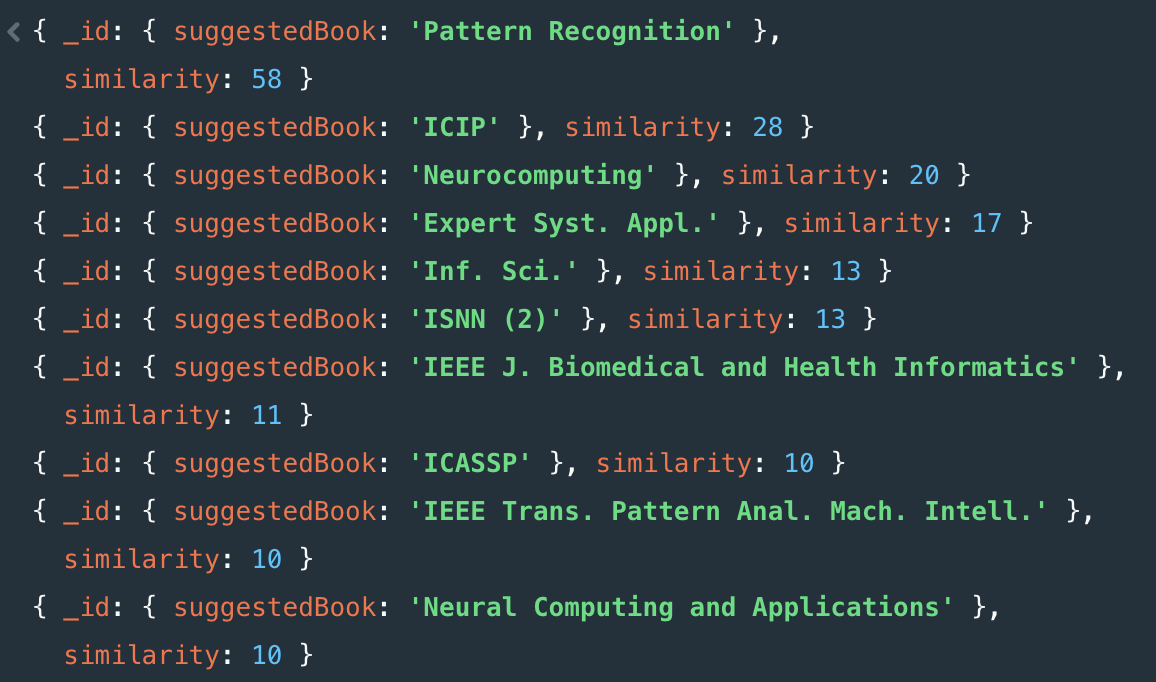
\includegraphics[width=0.9\linewidth]{ImagesMongoDB/query10mongodb}
            \label{fig:query10mongodb}%
        \end{center}
    \end{figure}
    \item \textbf{Authors who have referenced themselves the most within their papers} \\
    The query returns the authors who have referenced themselves the most.
    An author does a self-reference when the considered paper presents a reference to another paper the author has written.
    The results are the name of the authors and the number of times they have made a self-reference, the output is ordered using this number.
    \begin{lstlisting}[label={lst:query11mongodb}]
db.bibliography.aggregate( [ {
    $unwind: { path: "$references" } }, {
    $lookup: {
        from: "bibliography",
        localField: "references",
        foreignField: "_id",
        as: "referencedPaper" } }, {
    $match: { $expr: { $gt: [ {
        $size: "$referencedPaper" }, 0 ] } } }, {
    $unwind: { path: "$referencedPaper" } }, {
    $match: { $expr: { $ne: [
        "$_id",
        "$otherPaper._id" ] } } }, {
    $match: { "authors": { $exists: true } } }, {
    $match: { "referencedPaper.authors": { $exists: true } } }, {
    $unwind: { path: "$authors" } }, {
    $unwind: { path: "$referencedPaper.authors" } }, {
    $match: { $expr: { $eq: [
        "$authors", "$referencedPaper.authors" ] } } }, {
    $group: {
        _id: {
            authorId: "$authors._id",
            authorName: "$authors.name"},
        aut: { $sum: 1 } } }, {
    $sort: {"aut": -1} }, {
    $limit: 10 }, {
    $project: {
        "_id": 0,
        "name": "$_id.authorName",
        "autoreference": "$aut"} } ] )
    \end{lstlisting}
    \begin{figure}[H]
        \begin{center}
            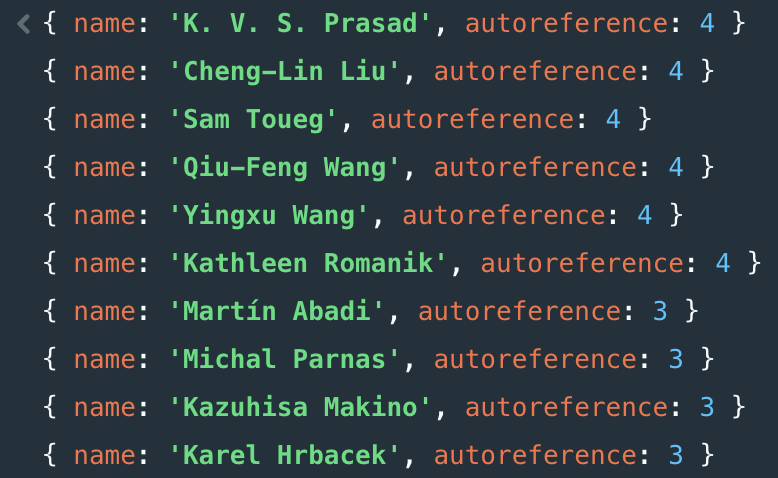
\includegraphics[width=0.6\linewidth]{ImagesMongoDB/query11mongodb}
            \label{fig:query11mongodb}%
        \end{center}
    \end{figure}
\end{enumerate}
